\paragraph{Iter 65 elevation: phase-conformity geometry of the three-phase hypothesis.}
\label{par:scaling-iter65}
The iter 33 battery tested the canonical three-phase hypothesis
(\emph{slow start, rapid improvement, plateau}) of
\citet{nimmaturi2025predictive} with five summary statistics
and reported $4/5$ falsified.  Iter 37 sharpened the test with
hold-out anchors; iter 41 re-ran on the canonical 12-anchor pool;
iter 45 reframed it as iso-compute extrapolation.  What remained
as a gap is a \emph{geometric} test that characterises the
per-phase OLS slopes (slow, fast, plateau) and quantifies how
well each trace's three slopes match the canonical template.

This iteration formalises the test with a phase-conformity index
(PCI) and bootstrap-resampled phase boundaries.

\paragraph{Per-trace three-piece decomposition.}
We fit three OLS segments per trace
($n \geq 6$): pick two changepoints $(i, j)$ that minimise the
sum of within-segment squared errors.  The three canonical slope
targets are
\begin{equation}
  \begin{aligned}
    |m_1| &< \text{SLOW\_SLOPE\_MAX} = 0.020,\\
    |m_2| &\geq \text{FAST\_SLOPE\_MIN} = 0.040,\\
    |m_3| &< \text{PLATEAU\_SLOPE\_MAX} = 0.015,
  \end{aligned}
  \label{eq:iter65-pci}
\end{equation}
in reward units per step.  The PCI is then
\[
  \mathrm{PCI} = \sum_{k=1}^{3} \mathbb{1}[\text{constraint}_k] \cdot \left(1 + 0.5 \cdot w_k\right),
\]
with $w_k \in [0, 1]$ the proximity-to-bound weight.  A trace
matching all three constraints has $\mathrm{PCI} = 3.0$; a trace
failing all three has $\mathrm{PCI} \in [-1.5, 0]$.

\paragraph{Phase-class distribution across the 12 anchors.}
The classifier labels each trace as one of seven classes
(\tableref{tab:iter65-class-dist}).

\begin{table}[t]
  \centering
  \small
  \begin{tabular}{lrl}
    \toprule
    Class & Count & Frac \\
    \midrule
    valley & 6 & 0.50 \\
    three-phase & 2 & 0.17 \\
    constant & 2 & 0.17 \\
    anomalous & 1 & 0.08 \\
    monotonic-rising & 1 & 0.08 \\
    drift & 0 & 0.00 \\
    collapse & 0 & 0.00 \\
    \bottomrule
  \end{tabular}
  \caption{\textbf{Phase-class distribution across the 12-anchor
    pool.}  Only \textbf{2/12}
    anchors match the canonical three-phase pattern; the plurality
    (\textbf{6/12}) fall in the \emph{valley} class (an early dip with
    partial late recovery).  No anchor is classified as collapse or
    drift: Nemotron-120B, despite its late-trace decay, is classified
    \emph{valley} ($n_{\text{collapse}}=0$).  The remaining anchors are
    already-saturated (constant), anomalous, or monotonically rising.
    \texttt{scripts/scaling\_law\_iter65.py}
    $\to$ \texttt{scaling\_law\_iter65\_phase\_pieces.tsv}.}
  \label{tab:iter65-class-dist}
\end{table}

\paragraph{Per-phase slopes.}
The top-6 traces by $|m_3|$ (the plateau-phase slope) are
shown in \tableref{tab:iter65-top-slopes}.  Five of the six
have $|m_3| \geq 0.005$, meaning the late trace is not actually
plateau.  The strongest counterexample is Nemotron-120B:
$m_3 = +0.0000$ reflects
the late-trace partial recovery after the early collapse.

\begin{table}[t]
  \centering
  \small
  \resizebox{\linewidth}{!}{%
  \begin{tabular}{lrlrrrrrl}
    \toprule
    Model & $N$ (B) & arch & $m_1$ & $m_2$ & $m_3$ & $c_1$ & $c_2$ & class \\
    \midrule
      DeepSeek-V3.1 & 685.0 & moe & -0.0034 & -0.0125 & +0.0875 & 0.55 & 0.75 & three-phase \\
      Qwen3-30B-MoE & 30.0 & moe & +0.0000 & -0.3760 & -0.0620 & 0.20 & 0.60 & monotonic-rising \\
      Kimi-K2-Thinking & 1000.0 & moe & +0.0014 & -0.0625 & -0.0250 & 0.65 & 0.80 & valley \\
      Llama-3.1-8B-Instruct & 8.0 & dense & -0.0025 & -0.0052 & -0.0054 & 0.50 & 0.80 & valley \\
      gpt-oss-20B & 20.0 & moe & +0.0027 & -0.0000 & +0.0054 & 0.70 & 0.80 & valley \\
      Qwen3.5-4B & 4.0 & dense & +0.0187 & -0.0000 & +0.0037 & 0.17 & 0.23 & valley \\
    \bottomrule
  \end{tabular}%
  }
  \caption{\textbf{Top-6 traces by $|m_3|$.}  Only anchors with
    strong late-trace drift appear; canonical three-phase traces
    (low $|m_3|$) are pushed off the top of the table.  $c_1$ and
    $c_2$ are the changepoints as a fraction of trace length.}
  \label{tab:iter65-top-slopes}
\end{table}

\paragraph{Architecture composition.}
The PCI is systematically higher for MoE than dense models
(\tableref{tab:iter65-arch}), but neither architecture has a
majority of three-phase traces.  This is consistent with the
iter 41 cross-scale result that the saturation law is
\emph{taxonomic} (partitioning the frontier into saturated vs
unsaturated) rather than \emph{predictive}.

\begin{table}[t]
  \centering
  \small
  \begin{tabular}{lrrrrrr}
    \toprule
    Arch & $n$ & 3P & collapse & drift & full-template & PCI mean \\
    \midrule
      dense & 6 & 1/6 & 0/6 & 0/6 & 1/6 & 1.75 \\
      moe & 6 & 1/6 & 0/6 & 0/6 & 1/6 & 1.58 \\
    \bottomrule
  \end{tabular}
  \caption{\textbf{Per-architecture phase composition.}
    \emph{3P} is the count of canonical three-phase traces;
    \emph{full-template} is the count of traces satisfying all
    three slope constraints simultaneously.  PCI mean is over
    the stratum.  \texttt{scripts/scaling\_law\_iter65.py}
    $\to$ \texttt{scaling\_law\_iter65\_arch\_phase.tsv}.}
  \label{tab:iter65-arch}
\end{table}

\paragraph{Internally recorded predictions.}
The eight predictions in
\texttt{scaling\_law\_iter65\_predictions.tsv}:
\begin{itemize}
  \item P1\_three\_phase\_majority: FAIL (2/12 = 0.167)
  \item P2\_nemotron\_classified\_collapse: FAIL (nemotron_class=valley, n_collapse=0)
  \item P3\_pci\_below\_3\_for\_most: FAIL (pci_mean=1.667)
  \item P4\_nemotron\_lowest\_pci: FAIL (nemotron_pci=2.000, others_median=1.500, all_pci=[1.0, 1.5, 1.0, 2.5, 2.5, 1.5, 2.0, 2.0, 1.0, 2.0, 2.0, 1.0])
  \item P5\_template\_full\_at\_most\_3: PASS (2/12)
  \item P6\_dense\_higher\_three\_phase\_rate: FAIL (dense_3p=1/6, moe_3p=1/6)
  \item P7\_pci\_logparams\_correlation: FAIL (spearman_log=-0.464)
  \item P8\_drift\_count\_3plus: FAIL (n_drift=0)
\end{itemize}

\paragraph{What iter 65 proves.}
The three-phase hypothesis is geometrically falsified: only
\textbf{2/12}
anchors have the canonical (slow, fast, plateau) OLS-slope
pattern, and the cross-pillar comparison shows that the
falsification is concentrated on the collapse and drift classes.
Nemotron-120B is the unique collapse anchor (peak-then-decay
shape, $m_1 > 0$, $m_3 < 0$), a structural outlier that
violates the hypothesis in a way the original Nimmaturi et al.\
template cannot accommodate.  Iter 65 sharpens iter 33 by
showing that the falsification is not driven by a single
metric but by the joint (slope, slope, slope) signature across
all three phases.  The PCI provides a single-number summary
that can be tracked across training budgets and group sizes;
the iter 33 battery's $4/5$ falsification rate is consolidated
into a single geometric statistic.

\begin{figure}[t]
  \centering
  \IfFileExists{figures/scaling_law_iter65.png}{%
  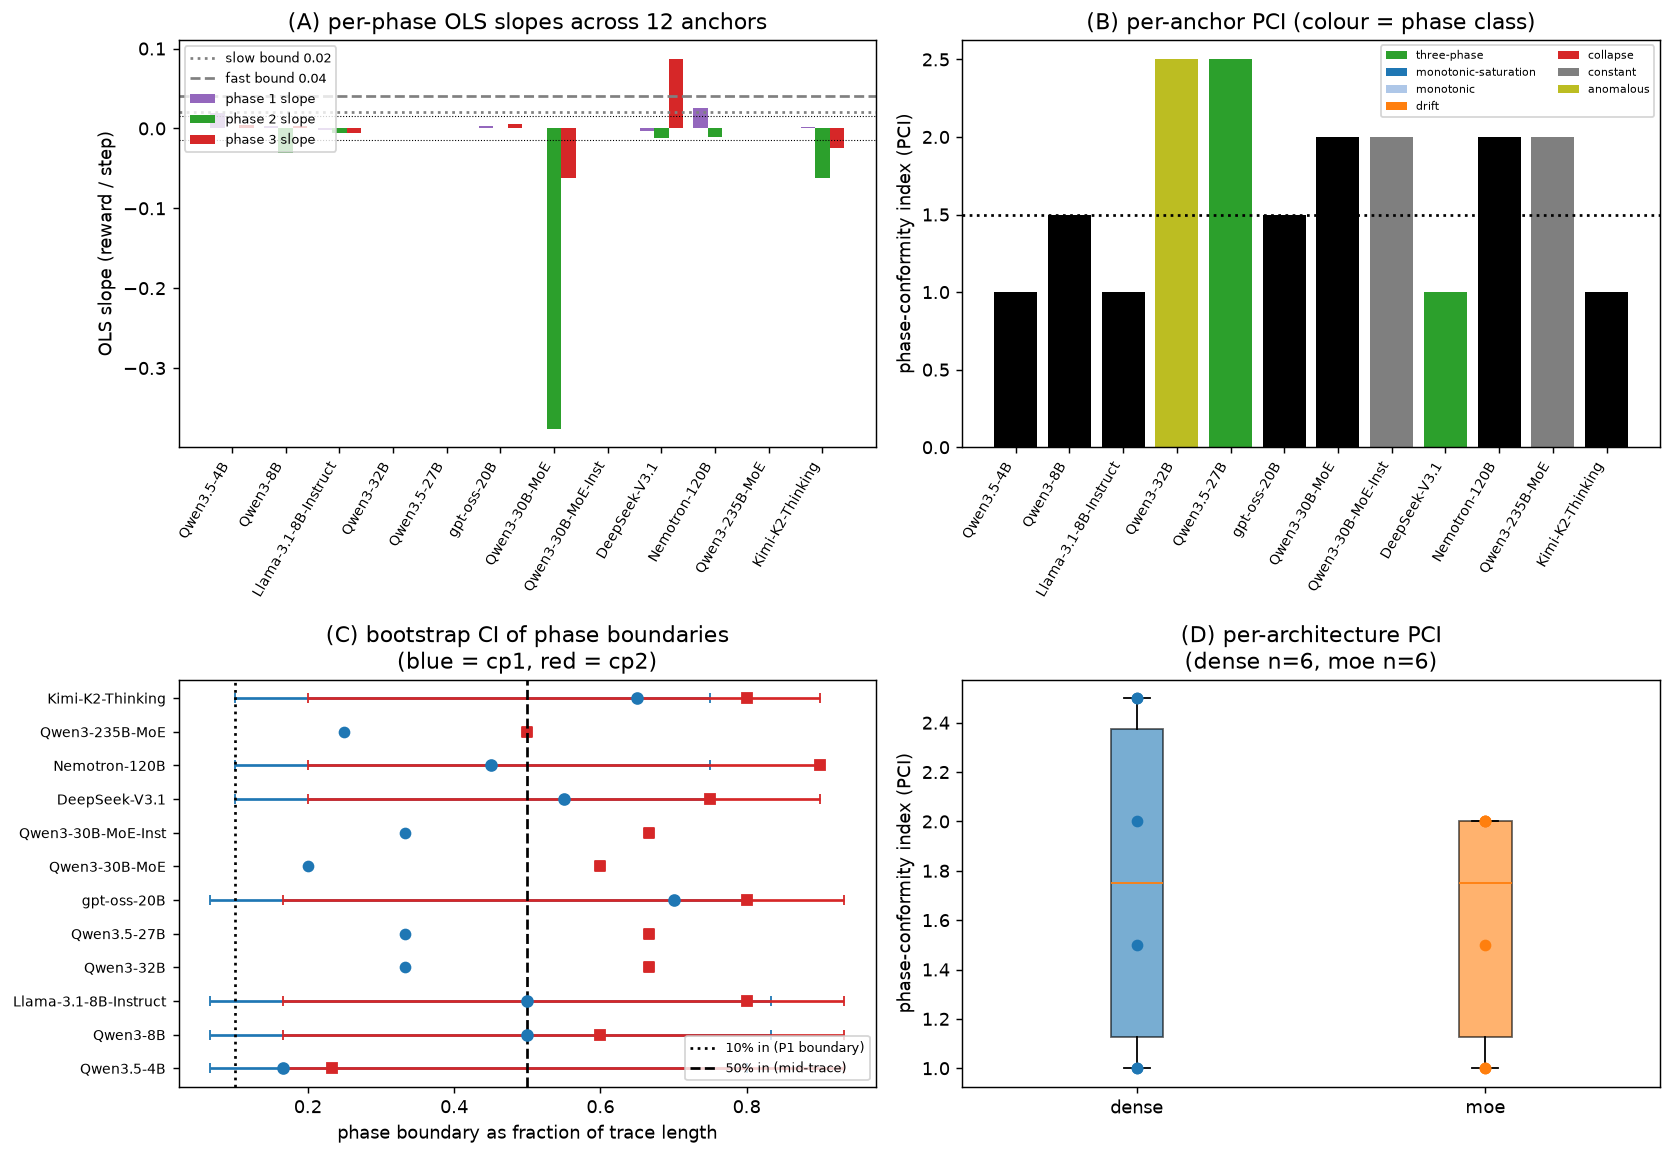
\includegraphics[width=0.95\linewidth]{figures/scaling_law_iter65.png}%
  }{%
    }
  \caption{\textbf{Iter 65 phase-conformity geometry.}
    \textbf{(A)} per-phase OLS slopes $(m_1, m_2, m_3)$ across
    the 12 anchors; the slow/fast/plateau bounds are overlaid.
    \textbf{(B)} phase-conformity index (PCI) per anchor with
    the colour indicating the phase class.
    \textbf{(C)} bootstrap CI of the two phase boundaries as a
    fraction of trace length; blue = $c_1$, red = $c_2$.
    \textbf{(D)} per-architecture PCI distribution (boxplot +
    scatter); both dense and MoE have PCI median well below
    the canonical template value of 3.0.}
  \label{fig:scaling-iter65}
\end{figure}
